\chapter{Trust in Vehicular Ad-hoc Networks}
\label{chap:vanets}

Today, most premium vehicles come equipped with hardware that allow for connectivity features; it is expected that, by 2022, many standard vehicles will also come with such features built-in, accounting for a substantial share of the automotive industry's revenue \citep{connectedcar2016}.
Although these features can be useful tools to aid drivers, reducing traffic and risk of accidents, they are merely a gateway to the long-term goal of truly autonomous vehicles, which might become a reality within the next decade; many automakers and technology companies have laid out their plans for the upcoming years \citep{tesla2016}.
However, the proper functioning and utility of both connected and fully autonomous vehicles rely on technologies, protocols and applications that allow for the fast communication between vehicle's on-board computers.

Vehicular ad-hoc networks, which are a special instance of MANETs, are a much-studied solution to the problems in the way of smart and autonomous vehicles.
In these networks, all nodes are related to traffic; they can be vehicles equipped with on-board computers, or stationary units placed near roads.
By quickly sharing data with neighboring vehicles, without the need of an Internet connection, smart vehicles can alert their drivers of important road conditions \citep{barba2012smart}, while autonomous vehicles can synchronize their movements to maximize traffic throughput \citep{amoozadeh2015platoon}.

%The advantages of an ad-hoc approach, as opposed to using cellular infrastructure or other server-based solutions, are explained in \autoref{chap:introduction}.
%For messages to travel to nodes out of the sender's wireless range, they must use other nodes as \textit{hops}.
%This approach requires appropriate routing protocols that consider the dynamic topology of VANETs.
%While traditional MANETs often use protocols which rely on the network topology, the ones proposed for VANETs generally use geographic position instead \citep{saini2015close}; these protocols use GPS coordinates in order to send messages to the available neighbor physically closest to the destination node.

%Certain cars available for purchase today are able to achieve some of those features (including autonomy) through a variety of sensors (cameras, accelerometers, microphones, etc.) which capture information about the world around them.
%However, these sensors don't provide a complete solution, since they are subject to a variety of interferences.
%The combination of built-in sensors with connectivity may provide the 

%The prospect of autonomous vehicles makes the study of Vehicular Ad-hoc Networks (VANETs) important.
%However, it will still take many years before completely autonomous vehicles are the norm and, until then, VANETs can be a valuable tool to help drivers reduce travel times and diminish the risk of collisions.
%Thousands of people die each year due to traffic accidents, many of which could have been avoided if vehicles were smarter and able to provide important alerts both to their drivers and to neighboring vehicles.
%The vehicles' on-board computers can aid drivers to increase safety and reduce traffic, but data needs to be shared among the various vehicles in the network.
%Such data includes location, speed and destination, which neighboring vehicles can use to adjust their trajectory and increase their own efficiency.
% By allowing vehicles to share their locations, speeds, and destinations with each other, traffic can become more stable and predictable.

\begin{figure}[h]
    \centering
    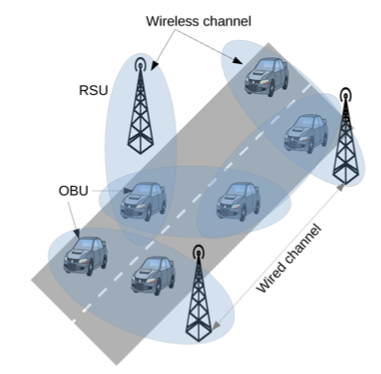
\includegraphics[width=0.5\textwidth]{images/vanet.png}
    \caption{Basic elements of a VANET: OBUs and RSUs. \citep{saini2015close}}
    \label{fig:vanet}
\end{figure}

Several current efforts to make VANETs viable in cities are centered around the IEEE 802.11p standard, also called Wireless Access in Vehicular Environments (WAVE) \citep{jiang2008ieee}.
Among other aspects of the wireless technology, the WAVE standard describes two types of nodes for vehicular networks: on-board units (OBUs) and road-side units (RSUs).
On-board units are computers placed within each vehicle which monitor the vehicle's data and are able to communicate with other nodes using wireless signals.
Road-side units are placed in static locations near roads; they may also have wired interfaces with other RSUs and the Internet, so it is possible to use them as anchor points for Internet access for passing vehicles.
When referring to the communication between two OBUs, the term vehicle-to-vehicle (V2V) communication is used \citep{yang2004vehicle}; when both an OBU and an RSU are involved, it is called vehicle-to-infrastructure (V2I) communication \citep{chou2009feasibility}.
Although this nomenclature is important to understand other studies on the subject of VANETs, this study does not consider RSUs and focuses only on vehicles themselves as nodes, so references to VANETs and vehicular networks are exclusively tied to V2V communications.

%When referring to VANETs, the terms vehicle-to-vehicle (V2V) and vehicle-to-infrastructure (V2I) are used.
%Both are types of communications that may occur within vehicular networks, depending on which nodes are actively participating in the networks.
%Aside from the vehicles themselves, VANETs can use road-side infrastructure to provide additional features, such as Internet access, to its users.
%In the model proposed in this work, however, such infrastructure is not used, so references to VANETs and vehicular networks are exclusively tied to V2V communications.

%[description of trust in context of VANETs]

In traditional networks (ad-hoc or not), routing protocols usually use the topology to choose where to forward packets; in other words, the primary metric used is the number of hops required to reach the destination.
This metric is not as useful in vehicular networks, since the high mobility causes the topology to change frequently.
Instead, most VANET routing protocols use geographical coordinates to forward packets \citep{saini2015close}, that is, the physical distance between two nodes is used as the primary metric.
The implication is that, even if a packet requires more hops to reach its destination, it will always be traveling the generally correct direction.

%[Explain basic security features]

As expected for a new technology being introduced, vehicular communications can become an appealing target for malicious users and attackers.
These are some examples of possible issues in a VANET:

\begin{enumerate}
	\item 	Vehicles with faulty GPS modules, speedometers or other sensors.
			If a vehicle is broadcasting incorrect data (perhaps unknowingly) because of a hardware or software fault, it can be a serious hinderance to efficiency and safety applications.
			It might behaving appropriately according to protocol, but the data it sends is not reliable \citep{isaac2010security}.
	\item	Vehicles might be deliberately broadcasting false data.
			In this case, there might be a specific purpose (by either the vehicle's driver or a remote attacker), like altering traffic or even cause an accident \citep{golle2004detecting}.
	\item   Attackers with control of several vehicles can propagate junk data in an attempt to flood the network, causing a distributed denial of service (DDoS) attack.
			Alternatively, the data propagated might have some reasoning behind it, like lying about road conditions in order to divert traffic \citep{garip2015congestion}.
	\item	Instead of sending data, some vehicles might try to eavesdrop on others' communications.
			The hop-based routing protocols used in VANETs facilitate this, since any node can be asked to be a hop.
			If the intermediary node is malicious, it may attempt to extract data contained in messages or refuse to forward them.
			Related to this, there is the Sybil attack \citep{isaac2010security}, in which a node lies about its position in order to seemingly alter the physical topology of the network and be chosen as a hop \citep{leinmuller2005influence}.
	\item	Malicious vehicles may use signal jammers or other devices in order to affect other vehicles' sensors and communications \citep{isaac2010security}.
			That can cause other vehicles to broadcast incorrect data, therefore obfuscating the origin of the attack.
	\item	A malicious user or remote attacker can monitor messages shared across the network in an attempt to stalk one specific vehicle \citep{isaac2010security}.
	
\end{enumerate}

Each of these possible attacks requires a unique approach, though there are some broader ways to help the security and safety of VANET users.
Trust, as is described in \autoref{section:trustvanet}, can be an important feature in vehicular networks, especially when attempting to filter out malicious or incorrect messages.
It does not, however, avoid all possible attacks, such as a signal jammer or stalking.
Rather, different mechanisms must be explored in order to avoid most problems.

%Related to trust is the issue of identity in vehicular networks.
%Solutions to this issue can be important elements of security and privacy, and there are studies focusing on node identification in VANETs (that is, making sure a node is who it claims to be), in particular through the use of a Public Key Infrastructure (PKI) \citep{wasef2010complementing}.
%In fact, at least one study proposes that these identities must be refreshed with a certain frequency to maintain the privacy of each node \citep{golle2004detecting}.
%However, refreshing identities can make maintaining a trust relationship between two nodes difficult or even impossible, since there is no way to know which nodes changed identities.
%Although it is important that nodes are not able to lie about identity and are able to maintain their privacy, persistent identities is a prerequisite for the model proposed here.

% While certification of identity is an issue in vehicular networks, and , this work will not address it.
%There are studies focusing on node identification in VANETs (that is, making sure a node is who it claims to be), in particular through the use of a Public Key Infrastructure (PKI) \citep{wasef2010complementing} 
%\citep{kumar2015intelligent}.
%One study proposes that such identities must be refreshed with a certain frequency to maintain the privacy of each node \citep{golle2004detecting}.
%Although it is important that nodes are not able to lie about identity and are able to maintain their privacy, nodes having valid identities that are persistent over time, so that nodes can identify each other over a long period, is a prerequisite for the model proposed here.


\section{Special properties of VANETs}
\label{section:properties}
%As was described above, VANETs are a special type of MANETs, which in turn are technological networks.
%However, 
VANETs feature several unique properties which distinguish them, and the behavior of its members, from other types of networks \citep{yousefi2006vehicular}.
Some of these properties include:

\begin{enumerate}

	\item 	Rapidly changing topology.
			Since the nodes are vehicles, they move frequently and at relatively high speeds.
			Each node's wireless communications also have a certain range, so the other nodes within that range (and, therefore, network neighbors) can change very quickly.
%			To build a topology model of its surrounding network, a node must often ping its neighbor to gather information.
%			Using velocity and location information, however, it is possible to create reasonable assumptions about future states of the topology.
			
	\item	Node mobility is constrained to a pre-existing grid of roads.
			Within those roads, nodes usually travel in predictable directions according to local laws and historical data.
			The spaces in the grid, like city blocks, provide a challenge to communication both because of distance and because buildings can cause obstructions to radio transmissions.
			
	\item	VANETs are prone to fragmentation, since a gap in the network topology can make two parts of it unable to communicate with each other.
			Combined with the property above, this fragmentation can appear and disappear frequently, depending on the node density.
			
	\item	Due to the changing topology and possible disconnection, connection with distant nodes is not reliable.
			Therefore, the effective diameter of the network is relatively small for important applications.
			
	\item 	Compared to devices like smartphones, vehicles have no notable power constraints.

	\item 	In certain locations and/or moments, large vehicle density results in a large-scale network, since there are many nodes concentrated in a relatively small space.
	
	\item 	The topology is susceptible to driver behavior.
			First, this means the topology can occasionally change in unpredictable ways.
			Second, contents of a message sent through the network can alter the driver's behavior and therefore change the topology.
			
\end{enumerate}

Some of these properties provide advantages or disadvantages when developing trust models for vehicular networks, although all of them must be considered.

\section{Trust in VANETs}
\label{section:trustvanet}
Like in other types of networks, the proper functioning of a VANET depends on the reliability of the vehicles (nodes) which participate in it.
If a node is malicious or faulty, it can spread incorrect data that may compromise the network's utility.
Once the concept of VANETs was established, researchers have been attempting to predict ways in which malicious users might use the network to their advantage.
Examples include triggering false alarms about inexistent accidents, lying about the average speed in a road to make it less desirable for others, and falsifying geolocation data to exploit location-based routing algorithms.
Therefore, the concept of trust must be established in the vehicular network context, allowing for nodes to judge the validity of information transmitted by others and share those conclusions with other nodes.

There is an important distinction between a malicious node and a faulty one; both of them may be sharing false data, but for different reasons and with different consequences.
For example, a malicious node may lie about its location in order to make routing protocols use it \citep{leinmuller2005influence}, in order to try to store or alter messages, while a faulty GPS module may cause an accident because its position data was incorrect.
However, that distinction can be hard to make, because a close inspection is necessary to determine whether the incorrect data is erratic or deliberate.
Since both types of nodes are problematic to the proper functioning of a network, malicious and faulty nodes can be treated as the same in a trust model.

%\textbf{/*********}
%Trust can be a related, yet distinct, issue to cryptography and authentication in vehicular networks.
%Many studies propose the use of a PKI (Public Key Infrastructure) to guarantee legitimate identities for nodes, although this solution requires, by definition, a certifying authority to manage and distribute public keys.
%VANETs must be able to function in a completely independent fashion, regardless of the amount of active nodes in a given region, and without relying on a centralized service.
%Both trust and authentication must work together to provide an adequate solution for VANETs, since it is difficult to establish trust without means to verify an identity (a malicious node may provide false data about its identity to bypass trust solutions), while a cryptography system requires a pre-existing infrastructure and may add unacceptable latency to high-priority messages.
%\textbf{[moved to chapter 4]}
%\textbf{*********/}

In general, trust management solutions for VANETs use \textit{data-oriented trust}, \textit{entity-based trust}, or a combination of the two.
The solutions that use data-oriented trust (or \textit{data-centric trust}) \citep{raya2008data} focus on validating messages instead of entities.
This is important when vehicles share messages about a specific event, such as a collision, which must be quickly validated by neighbors and distributed to other nodes within a relevant area.
In this scenario, vehicles sharing the same road might be complete strangers to each other, and therefore would not have any trust relationship, so neighboring nodes must decide if a message is true by its contents and by other nodes' observations of the event.
On the other hand, when dealing with frequent messages which contain basic information such as geolocation and speed (used for traffic-diminishing solutions), it is too costly to judge each individual message.
Therefore, \textit{entity-based trust} becomes more appealing, since benign nodes can quickly identify a malicious node and isolate it from the network.
% These models take advantage of the possibility of nodes meeting more than once and, therefore, being able to form a long-term trust relationship with each other.
Within entity-based trust, there are also two often-used methods of establishing trust: first, there is \textit{role-based trust}, which is the static trust of pre-authenticated vehicles such as police units; second, there is \textit{experience-based trust}, which is built through previous encounters shared between pairs of nodes.
The model proposed in this work utilizes entity-based and experience-based trust, as it is based on the possibility of nodes meeting more than once and, therefore, being able to form a long-term trust relationship with each other.
%It is not, however, mutually exclusive to other solutions 

%\textbf{/*********}
%In \citep{gerlach2007trust}, the author shows a general framework of how security and trust can be organized in a vehicular network.
%It proposes three layers: a service plane, which contains the core functionalities of the network, such as communication technologies, routing algorithms and the security measures directly related to them (such as cryptography); a middleware plane which handles trust and privacy issues; and the application layer, which contains the applications that will use the other layers' data to make decisions.
%The model shows neatly how security and trust can interact with each other to provide best results.
%\textbf{*********/}

%[malicious and faulty nodes]

%[details of security and safety issues in VANETs that can be diminished by trust]
\section{Desired properties for VANET trust models}
\label{section:properties}

The analysis of related work is based on \citep{zhang2011survey}, which proposes eight desired properties for a trust management model for VANETs.
In this section, these properties are briefly described.
% with an assessment of whether or not TruMan satisfies their conditions.
%\autoref{table:properties} shows how well TruMan and previous work satisfy the properties.

\textit{1. Decentralized trust establishment}: nodes must be able to form their own trust values about other nodes without the aid of an Internet connection or centralizing agents.
Nodes may or may not use information from other trustworthy nodes to build trust values (in other words, trust might be transitive).
%TruMan satisfies this as it is built from the ground up for decentralized systems.

\textit{2. Coping with sparsity}: the model still functions when there are few nodes populating the network.
Due to the dynamic nature of vehicular networks, it is possible that nodes will find themselves with few other nodes in range.
In such scenarios, a trust model should be able to establish trust even if there are few neighbors with whom to share data.
%In some cases, this can be achieved by using information that is immediately available; for example, if a vehicle broadcasting information happens to be a certified ambulance, its role is enough to guarantee trust.
%In other cases, models must consider solutions similar to delay-tolerant networks: storing information as it is received and sharing it with other trustworthy nodes when possible.
%The experiments using low density values demonstrate that TruMan works in reasonably sparse networks.
%Due to its decentralized nature, it can also work on isolated chunks of the network.

\textit{3. Event/task and location/time dynamics}: the model reacts to different situations depending on what, where and when events happen.
The event or task dynamics involve managing different situations in different ways.
Messages can carry different types of alerts, and not all of them need to be addressed with the same urgency.
A message about a nearby crash, for example, requires a much quicker reaction than one about an upcoming change in weather; malicious nodes that broadcast false information about critical events are especially important to detect.
Similarly, in order to satisfy location and time dynamics, nodes might behave differently according to where and when certain messages are received.
To do this, messages about events must contain timestamp and geolocation data attached; nodes close to the event in space and in time could be considered more trustworthy. 
Furthermore, by attaching timestamp data to messages, it is possible to age information, allowing the model to consider only data that is recent enough to be relevant.
%Although this has not been used in the simulations in this paper, TruMan can easily be extended to consider time and location as long as nodes store geolocation and timestamp data.

\textit{4. Scalability}: the model can work on very large networks at high speeds.
This is very important in vehicular networks, since, at certain times or locations, there might be a very large number of vehicles very close to one another. 
%In order to attain scalability, a model may consider limiting the volume or frequency of trust-related messages a node can receive at a given moment.
In the case of a model that allows transitive trust, a high volume of nearby vehicles can be advantageous because it allows nodes to share a lot of recent data with each other.

%Due to the low complexity of the algorithms used in the model, TruMan can be highly scalable, as it does not incur substantial pressure on the vehicles' on-board units.
%It has also been demonstrated that iterations of the algorithm do not need to run extremely frequently in order to detect malicious nodes with high accuracy.

\textit{5. Integrated confidence measure}: allows nodes to estimate how useful the output of the algorithm is.
Along with the information of whether or not a node $a$ trusts $b$, there should also be information regarding \textit{how sure} $a$ is of its trust in $b$.
Generally, a higher confidence measure is the result of more and/or better evidence.
%Since nodes using TruMan store trust values as a number between 0 and 1, this value can be used as a confidence measure of the opinion.
%The closer it is to 1, the higher the chance that it is accurate.

\textit{6. System level security}: requires authentication of nodes participating in the network.
There should be an infrastructure in place in order to avoid identity falsification from potentially malicious nodes as well as verifying which node is the sender of a given message.

%A public-private key solution can be used to  allows nodes to verify that messages it received were truly sent by who claimed to send it.
%This has not been considered in evaluations of TruMan.
%However, it can be included as a separate security model during the transmission of messages.

\textit{7. Sensitivity to privacy concerns}: avoids eavesdropping and stalking by malicious nodes.
A message should only be received by the nodes it was meant for, avoiding eavedropping of its contents.
Additionally, it should not be possible to track the activity of a node based on the messages it sends.

%TruMan has not been designed with this in mind, but it does not inhibit privacy protection.
%However, it does require that nodes cannot be completely anonymous.

\textit{8. Robustness}: the model's resistance to attacks.
There are already some studied attacks for vehicular networks, such as the Sybil Attack, Newcomer Attack and Betrayal Attack.
Models must show that they function in the event of such attacks.
%TruMan satisfies this property. Malicious nodes are quickly and accurately identified, making it difficult for them to perform attacks.
%Experiments show that, when fewer than 50\% of nodes in the network are malicious, Truman performs as expected.
%Collusion attacks must be performed by more than half of the entire network, in which case the network is considered compromised.
%Furthermore, since nodes take into consideration experiences from other trustworthy nodes, a malicious node that occasionally behaves correctly can still be identified. 
%Furthermore, the analysis also takes into account the complexity of the algorithm necessary to implement the trust model, because a high priority of TruMan is the 

%Finally, it is worth noting that, considering the scale of the problem, TruMan's cost is very low without sacrificing completeness and correctness.
%The model still satisfies or permits most of the desired properties of a trust model, making it viable for real-world use.

\section{Existing trust models for VANETs}
 
Several models have been proposed to solve the problem of trust in vehicular networks. 
In this section, the most relevant ones are described, considering the time in which they were proposed, the advantages they bring and their contributions to later study. 
None of them provide a complete solution, but serve as pieces of a puzzle that is still incomplete. 
Many trust management solutions for VANETs have been proposed over the years, such as \citep{patwardhan2006data}, \citep{gerlach2007trust}, \citep{raya2008data}, \citep{huang2010situation}, \citep{ding2013novel}, \citep{haddadou2013trust}, \citep{liu2016lsot}, \citep{kerrache2016detection}.
There are also some review and/or survey articles on the subject of VANET trust models, such as \citep{zhang2011survey}, \citep{ma2011survey}, \citep{zhang2012trust}, \citep{mejri2014survey}, \citep{soleymani2015trust} \citep{sengar2016survey}, and \citep{dwivedi2016review}. 

\citep{dotzer2005vars} is one of the earliest examples of VANET trust models, establishing a system called VARS, based on the reputation of nodes and messages throughout the network.
The authors use what they call \textit{opinion piggybacking}, which means that, for each hop between the origin and the destination of an event-related message, the forwarding node appends its opinion of the message's contents and the message's sender.
In other words, when a node $a$ receives a message about a certain event from $b$, it calculates a new opinion considering  it rebroadcasts the message to other nearby nodes, but with its own opinions about the event and about node $b$ attached.
%That opinion is formed using a combination of the forwarding node's own observations of the event, its opinion of the origin node and previous opinions appended to the message.
This process adds credibility to a message through validation by nodes in a decentralized fashion.
It combines aspect of data- and entity- based trust, since nodes share their opinion of the data as well as their opinion of the sender. 
An interesting observation is setting higher trust values for certain vehicles based on their familiarity with the region (vehicles that reside in a given city may have more experience with certain types of events than newcomers).
However, opinion piggybacking has its own share of problems.
First, it allows forwarding nodes to access (at least some of) the contents of a message so it can form an opinion on it, diminishing privacy; a malicious forwarding node could even attempt to alter those contents.
Second, since each new opinion appended to the message considers the previously appended opinions, the first nodes to forward the message to have a substantially greater impact over the final opinion than the later ones.
Finally, there is an issue with scalability, since appending new information to a message on each hop may add a significant overhead to the transmission. Additionally, the authors provide little to no experimentation or proof that their approach would be sound in a real-world network.

The model proposed in \citep{minhas2010towards} uses several criteria to judge whether or not a received message is trustworthy.
First, nodes are classified by their roles and previous experience with them.
Roles are used for vehicles which should be more trustworthy than the average: government official cars, traffic report vans, buses, cabs, etc.
Nodes also store their experience each time an event message is received (if one neighboring node reported an event which did not turn out to be true, its trust value is reduced).
Additionally, messages have higher reliability when their senders are closer in time and space to the reported event.
When several messages about the same event are received, a node can either choose the $n$ most trustworthy senders, according to the priority (fewer chosen nodes means a faster, but less precise, decision), or compute the majority opinion of the messages according to each sender's trust value.
The model considers both role-based trust and experience-based trust; although the work proposed here does not use role-based trust, the authors provide a useful method of calculating and updating an experience-based trust value, which might be used or adapted.
However, their model relies only on direct interaction between pairs of nodes, so no form of indirect trust (that is, trust values received from other nodes) is considered.

%Although the model proposed here will not take role-based trust into consideration and does not emphasize event-related messages, the author's approach to experience-based trust resembles what will be described in \autoref{chap:proposal}.

In \citep{chen2010trust}, the authors propose to evaluate messages utilizing a cluster-based trust model.
By separating nodes into clusters with their geographical neighbors, it is possible to efficiently distribute the evaluation of messages using previously formed opinions.
When a node sends a message, one node in the cluster (the leader) must aggregate the other nodes' opinions on that message.
Afterward, the message is only forwarded to another cluster if that aggregate opinion is above a certain threshold; furthermore, nodes that receive the message only act upon it if the overall trust on it is above another threshold, which can be different according to the nature of the message.
However, it is unclear how the model behaves when the network is too sparse to form relevant clusters, neither do the authors inform how the aforementioned thresholds are decided.
Furthermore, maintaining clusters in a highly dynamic network is a costly job and, if the cluster leader itself is malicious, all the information from that cluster becomes untrustworthy.
%The whole premise of organizing a VANET in clusters is  
%The model considers role-based trust (i.e. static trust of pre-authenticated vehicles such as police units) and experience-based trust, which is calculated using knowledge of the outcomes related to previous messages.
%This model considers both role-based and experience-based trust.

The trust model in \citep{park2011long} takes advantage of daily commutes.
In this article, the focus is on the early stages of VANETs, in which a very small percentage of vehicles are equipped with OBUs.
To make trust viable in such a scenario, the authors rely on RSUs to store reputation information from passing vehicles.
Each vehicle must have an ``Agent RSU'', which is in charge of storing and sharing that vehicle's trust data to other passing vehicles and connected RSUs.
It must also keep the data updated when the vehicle approaches it again.
To make this viable, the properties of daily commutes are used: it is assumed that the vehicle is near its Agent RSU with reasonable frequency because it is located within the driver's home-to-work route.
The main problem with this model is that it relies on the presence of frequent RSUs, which might not always be viable.
It also does not make it clear what should happen when a vehicle stops using a route or does not have a daily predictable path (it does, however, handle occasions in which a vehicle chooses an alternate route or is absent for some days such as weekends and holidays).

The authors of \citep{huang2014social} take special note of two characteristics from social networks that can also be found in many VANET trust models: \textit{information cascading} and \textit{oversampling}.
That is, information reported by a number of original nodes (i.e. the ones that witnessed an event) may be diluted as nodes that forward it append their own opinions on the matter.
An algorithm is proposed to diminish that effect by assigning higher weights to the opinions of origin nodes and lower weights  to others.
However, the authors conclude that the optimal scenario is to assign no weight at all to forwarding nodes, therefore allowing each node to form an opinion based only on the original nodes' reports.
Furthermore, the authors are quick to dismiss the validity of entity-based trust, instead opting for a pure data-oriented approach.
%Since their model is based only on events, it also does not consider the usefulness of trust in more mundane cases such as the frequent sharing of location and speed among vehicles.
Although it is true that data-oriented trust is efficient for events, which is what their model is based on, it is not ideal for sharing data quickly and frequently.
When a collision or other major incident occurs, it is useful to judge each message on its own, since not all members of the network will have existing trust relationships with each other.
However, when sharing location and velocity data several times per second, it is not reasonable to expect that each message will be analyzed so carefully; rather, it makes sense to form an opinion about the sender of the message and use the resulting trust value to choose which messages are relevant or not.

The Attack-Resistant Trust Management Scheme (ART) from \citep{li2016art} proposes to resist three types of attacks: 
simple attacks, in which malicious nodes do not cooperate with the network;
bad-mouth attacks, in which malicious nodes perform simple attacks but also share false information about benign nodes;
and zig-zag attacks, in which nodes vary their behaviour from benign to malicious in order to be harder to detect.
It works in two main steps: data gathering and malicious node detection.
For data gathering, it uses the Dempster-Shafter theory of evidence, which establishes \textit{belief} and \textit{plausibility} values, both real numbers ranging from 0 to 1.
The former refers to the amount of evidence indicating the truthfulness of a hypothesis (for example, a node sending false data corroborates the hypothesis of it being malicious), while the latter is 1 minus the amount of evidence that supports the possibility of the hypothesis being false.
These evidences are acquired through observations by a node and through data received from other nodes.
The resulting probability is the basic trust value, which is stored in a trust vector (a series of trust values regarding other nodes).
The malicious node detection step uses a Cosine-based metric to compare two nodes' trust vectors.
When two nodes share similar opinions about other nodes, they will consider each other trustworthy.
The downside of this model is that each step is mathematically costly, requiring several intensive calculations in order to achieve its goals.
This likely increases the complexity of the algorithm, which is not detailed by the authors.
Because of this, it is uncertain how the model would scale to large networks, while it might also underperform in small networks in which there is little evidence to collect.
%The authors present no details on how it deals with sparsity, dynamics, scalability, security and privacy.
%extend

The authors of \citep{chen2017cloud} propose a cloud-based solution for a trust model, which requires an Internet-based global trust manager.
This has the advantage of simplifying properties such as handling sparsity and scalability, but also makes the system slower in general, especially in situations in which mobile communication is slow or unreliable.
In general, it goes against several established concepts for vehicular networks, such as being completely decentralized and ad-hoc.
It also makes the system somewhat, since the whole system collapses if the global trust manager is attacked, or could leave the network members unaided in the event of a server or connection failure.
%extend

%conclude
\autoref{table:properties} shows how well each studied trust model satisfies the eight properties described in \autoref{section:properties}.
The numbers used in the table are the same ones from \autoref{section:properties}.
This analysis shows that, although several previously proposed trust models provide reasonable solutions to the trust management problem, all of them have issues in terms of correctness, completeness or efficiency, indicating that the problem is not yet truly solved.

\begin{table}[t!]
\caption{Properties of the related work}
\label{table:properties}
\centering
\begin{tabular}{|p{4cm}||p{0.5cm}|p{0.5cm}|p{0.5cm}|p{0.5cm}|p{0.5cm}|p{0.5cm}|p{0.5cm}|p{0.5cm}|}
 \hline
 \textbf{Property} & 1 & 2 & 3 & 4 & 5 & 6 & 7 & 8\\
 \hline
 \hline
% TruMan & \checkmark & \checkmark & \checkmark & \checkmark & \checkmark & - & - & \checkmark \\
% \hline
% \citep{vernize2015malicious} & 1 & 2 & 3 & 4 & 5 & 6 & 7 & 8\\
% \hline
 \citep{dotzer2005vars} & \checkmark & - & \checkmark & - & - & - & \checkmark & -\\
 \hline
 \citep{minhas2010towards} & \checkmark & \checkmark & \checkmark & \checkmark & \checkmark & \checkmark & \checkmark & -\\
 \hline
 \citep{chen2010trust} & \checkmark & \checkmark & \checkmark & \checkmark & \checkmark & \checkmark & - & -\\
 \hline
 \citep{park2011long} & - & - & - & - & - & \checkmark & \checkmark & \checkmark \\
 \hline
 \citep{huang2014social} & \checkmark & - & \checkmark & \checkmark & \checkmark & - & - & -\\
 \hline
 \citep{li2016art} & \checkmark & - & - & - & \checkmark & - & - & \checkmark\\
 \hline
 \citep{chen2017cloud} & - & \checkmark & - & \checkmark & - & \checkmark & \checkmark & -\\
 \hline
\end{tabular}
\end{table}

%\begin{table}[t!]
%\caption{Properties of Truman and related work}
%\label{table:properties}
%\centering
%\begin{tabular}{|p{3cm}||p{3cm}|p{3cm}|p{3cm}|p{3cm}|p{3cm}|p{3cm}|p{3cm}|}
% \hline
% \textbf{Property} & TruMan & \citep{vernize2015malicious} & \citep{minhas2010towards} & \citep{chen2010trust} & \citep{li2016art} & \citep{chen2017cloud} \\
% \hline
% Decentralized 	& \checkmark & -		  & \checkmark & \checkmark & \checkmark & - \\
% \hline
% Sparsity 		& \checkmark & -		  & \checkmark & \checkmark & -			 & \checkmark \\
% \hline
% Dynamics 		& \checkmark & - 		  & \checkmark & \checkmark & -			 & - \\
% \hline
% Scalability 	& \checkmark & \checkmark & \checkmark & \checkmark & -			 & \checkmark \\
% \hline
% Confidence 	& \checkmark & \checkmark & \checkmark & \checkmark & \checkmark & - \\
% \hline
% Security 		& -			 & - 		  & \checkmark & \checkmark & - 		 & \checkmark \\
% \hline
% Privacy 		& - 		 & - 		  & \checkmark & - 			& -			 & \checkmark \\
% \hline
% Robustness 	& \checkmark & -		  & -		   & - 			& \checkmark & - \\
% \hline
% Efficiency		& \checkmark & \checkmark & -		   & -			& -			 & - \\
% \hline
% Cost & $|V|*|E|$ & $|V|+|E|$ & n/a & n/a & n/a & n/a\\
% \hline
%% \hline
%\end{tabular}
%\end{table}


%\begin{table}[h!]
%\centering
%\begin{tabular}{ |p{3cm}||p{1cm}|p{1cm}|p{1cm}|p{1cm}| }
% \hline
% & Dotzer & Chen & Huang & Park\\
% \hline
% Decentralized   & AF    &AFG&   004 &\\
% \hline
%\end{tabular}
%\caption{Features of VANET trust models}
%\label{table:1}
%\end{table}



%=====================================================
